% !TEX encoding = UTF-8 Unicode
\documentclass[a4paper,10pt,spanish]{article}

\usepackage[T1]{fontenc}
\usepackage[utf8]{inputenc}
\usepackage{mathtools}
\usepackage{graphicx}
\usepackage[margin=1in]{geometry}
\usepackage[spanish,activeacute]{babel}
\usepackage{hyperref}
\usepackage{fancyhdr}
\pagestyle{fancy}

\usepackage{color}
\usepackage{listings}
\lstset{ %
language=Octave,                % choose the language of the code
basicstyle=\footnotesize,       % the size of the fonts that are used for the code
numbers=left,                   % where to put the line-numbers
numberstyle=\footnotesize,      % the size of the fonts that are used for the line-numbers
stepnumber=1,                   % the step between two line-numbers. If it is 1 each line will be numbered
numbersep=5pt,                  % how far the line-numbers are from the code
backgroundcolor=\color{white},  % choose the background color. You must add \usepackage{color}
showspaces=false,               % show spaces adding particular underscores
showstringspaces=false,         % underline spaces within strings
showtabs=false,                 % show tabs within strings adding particular underscores
frame=single,           % adds a frame around the code
tabsize=2,          % sets default tabsize to 2 spaces
captionpos=b,           % sets the caption-position to bottom
breaklines=true,        % sets automatic line breaking
breakatwhitespace=false,    % sets if automatic breaks should only happen at whitespace
escapeinside={\%*}{*)}          % if you want to add a comment within your code
}
\renewcommand{\lstlistingname}{Código}
\usepackage{float}
\restylefloat{table}
\makeatletter
\def\verbatim{\small\@verbatim \frenchspacing\@vobeyspaces \@xverbatim}
\makeatother

\title{Random Sparse Matrix}

\lhead{Métodos Numéricos Avanzados}
\rhead{Random Sparse Matrix}

\begin{document}

\begin{center}
\textbf{\Huge{Random Sparse Matrix}}
\end{center}

\vspace{10mm}

\begin{center}
\textbf{INTEGRANTES: Badi Leonel, Nicolas Buchalter, Franco Depascualli, Agustin Scigliano, Marco Fallone}

\textbf{ITBA Segundo Cuatrimestre 2015}
\end{center}

\begin{center}
\text{PALABRAS CLAVE: matriz rala, random sparse matrix, mvmran, matran, autovalores, descomposición qr}
\end{center}

\vspace{10mm}

\begin{center}
\begin{large}
Resumen
\end{large}
\end{center}

Las matrices de valores dispersos(RSM) son un tipo de matriz que poseen la particularidad de tener gran cantidad de valores iguales a ceros. Conceptualmente se pueden pensar como matrices que representan sistemas donde sus elementos tienen baja cantidad de conexiones entre si, por ejemplo una red de computadoras. En este informe nos enfocaremos a analizar solamente las matrices de valores dispersos aleatorios, construidas de tal manera que tengan la misma cantidad de elementos diferentes a cero en cada columna.

\section{Introducción}
En el siguiente informe detallamos una implementación en Octave para el cálculo de autovalores en matrices RSM. Primero describiremos la implementación realizada, las decisiones que se tomaron, las dificultades que se encontraron y posibles mejoras que se pueden realizar en un futuro.

\section{Metodología}
Se decidió implementar todos los métodos en Octave ya que posee varias herramientas útiles ya implementadas para realizar operaciones con matrices (por ejemplo el producto).
Si bien para almacenar estas matrices se pueden utilizar estructuras como listas de listas o representaciones como Yale(utilización de 3 vectores), se optó por representarlas utilizando las matrices de Octave para aprovechar las ventajas antes mencionadas. También, se pensó en almacenarlas utilizando una estructura y a la hora de operar realizar una conversión a matrices de Octave. Se desestimó esta idea por el costo de procesamiento que conlleva realizar conversiones constantemente.
Para obtener los autovalores se decidió utilizar el método iterativo de QR visto en clase, con la salvedad de que en este trabajo se contemplan los casos donde los autovalores son complejos. Para determinar en que momento hace falta calcular estos valores complejos se decidió utilizar doble shifteos.

Para la descomposición QR se implemento el método de GS visto en la clase, el método modificado de GS y el método de las rotaciones de Givens.

\subsection{Implementación}
\subsubsection{Generación RSM}

Para la generación de las matrices RSM primero se generan dos matrices, una de números aleatorios y de dimensión N x NZR, la otra de ceros y de dimensiones N - NZR x N.
Luego estas matrices se concatenan una debajo de la otra para formar una matriz de dimensiones N x N. Por ultimo se itera sobre todas las columnas y se permuta de manera aleatoria las filas utilizando la función randperm de Octave.
Se puede demostrar que el orden de complejidad de esta función es \[N  O ( randperm ) \].
\begin{lstlisting}[caption = Implementación del generador de matrices RSM]
	function ret = generateRSM(N,NZR)
		A = rand(NZR,N);
		B = zeros(N-NZR,N);
		A = [A ; B];

		% Shuffle the matrix
		for i = 1:N
			ret(:,i) = A(randperm(N), i);
		end
	end
\end{lstlisting}

\subsubsection{Método QR - GS}
Como se puede ver a continuación, se implemento el método de GS propuesto por la cátedra sin realizare ninguna modificación. Este método tiene la desventaja que como genera vectores de norma pequeña, puede llevar a errores grandes en los primeros pasos que luego son arrastrados y amplifican los siguientes.

\begin{lstlisting}[caption = Implementación de la descomposición QR con GS]
	function [Q,R] = custom_qr(A)
		n = length(A);
		Q(:,1) = A(:, 1) / norm(A(:, 1));

		for i = 2 : n
			u = A(:, i);
			for j = i-1  : -1 : 1
				u = u - A(:, i)' * Q(:, j) * Q(:, j);
			end
			Q(:, i) = u / norm(u);
		end
		Q = -1*Q;
		R = Q'*A;
	end
\end{lstlisting}
\subsubsection{Método QR - GS modificado}

A continuación se muestra el método modificado de GS.

\begin{lstlisting}[caption = Implementación de la descomposición QR con GS]
	function [Q,R] = modGS_qr(A)
		R = 0;
		m = size(A)(1);
		n = size(A)(2);
		for k = 1 : n
			R(k,k) = norm(A(1:m,k));
			Q(1:m,k) = A(1:m,k) / R(k,k);
			for j=k+1 : n
				R(k,j) = Q(1:m,k)' * A(1:m,j);
				A(1:m,j) = A(1:m,j) - Q(1:m,k) * R(k,j);
			end
		end
	end
\end{lstlisting}
\subsubsection{Método QR - Rotaciónes de Givens}

Dada una matriz cualquiera, se puede obtener una rotaciones de Givens tal que: \[  A=G B  \] siendo B igual a A pero con un elemento en 0. Este proceso se puede aplicar N veces para obtener una matriz triangular superior.
De esta manera podemos definir a Q como la aplicación de todas las transformadas de rotación \[ Q = G_n ... G_1  Id  \] \[ R = G_n ... G_1  A  \]

El método fue implementado siguiendo la propuesta de la cátedra, pero haciéndole una modificación para que se calcule correctamente Q.

\begin{lstlisting}[caption = Implementación de la descomposición QR con GS]
	function [Q,R] = givens_qr(A)
		R = A;
		m = size(A)(1);
		n = size(A)(2);
		Q = eye(m,n);
		for k = 1 : n
			for l = k +1 : m
				if (R(l,k) == 0)
					c = 1;
					s = 0;
				elseif abs(R(l,k)) < abs(R(k,k))
					t = R(l,k) / R(k,k);
					c = 1 / sqrt(1+t^2);
					s = c * t;
				else
					z = R(k,k) / R(l,k);
					s = 1/ sqrt(1 + z^2);
					c = s*z;
				end
				G = [c,s; -s,c];
				R([k,l] , k:n) = G * R([k,l], k : n);
				Q([k,l] , 1:n) = G * Q([k,l], 1:n);
			end
		end
		Q = Q';
	end
\end{lstlisting}




\subsubsection{Método eig}

Luego de implementar la descomposición QR, se prosiguió a implementar la funcion \texttt{eig}. 

Una vez implementada la descomposición QR, resultó sencillo implementar la función \texttt{eig} (Ver código 2). La función se implementó de manera recursiva tal como fue mostrada en la clase. El caso base de esta función es con una matriz de 2x2 ya que el cálculo de sus autovalores implica encontrar las raíces de un polinomio de grado 2. El paso recursivo consta en hallar la descomposición QR de la matriz  y hacer el producto entre R y Q.

Al momento en que la matriz converge, si los autovalores son reales se encontrarán en la diagonal. Si los autovalores son complejos, obtendremos matrices de dimensión 2 en la diagonal y se pueden obtener los autovalores conjugados de ellas. Si la matriz GRCAR es de dimensión impar habrá exactamente un autovalor real y este aparecerá en la última fila y columna de la matriz resultantes. Una matriz de dimensión par sólo tendrá autovalores complejos conjugados (ninguno real).

Como dijimos anteriormente, la precisión elegida para el cálculo de autovalores es de $10^{-4}$ por lo tanto, decidimos agregar un chequeo de los determinantes de la matrices de 2x2 que se forman en la diagonal y compararlos con los anteriores. Cuando la diferencia de todos los determinantes con sus respectivos antecesores se hagan menor que el error, el algoritmo retorna. De esta manera no es necesario que la matriz haga las iteraciones máximas para finalizar. Como dicho chequeo es costoso para matrices de gran tamaño, se utiliza una constante de frecuencia de chequeo para no tener que revisar el error en cada paso sino de a pasos mas grandes a medida que la matriz sea de mayor dimensión.

\begin{lstlisting}[caption = Implementación del algoritmo QR en Java]
public static List<Complex> eig(double[][] m) {
		List<Complex> eigs = new ArrayList<Complex>();
		if (m.length == 2 && m[0].length == 2)
			return Complex.roots(1, -m[0][0] - m[1][1], Vector.determinant(m));
		double [] dets = new double[(m.length)/2];
		double[][] T = m;
		boolean flag = false;
		for (int k = 0; k < MAX_ITERATIONS && !flag; k++) {
			Map<String, double[][]> qr = QR(T);
			T = matrixprod(qr.get("R"), qr.get("Q"));
			if( k % (m.length*CHECK_FREQUENCY) == 0){
				double[][] current = new double[2][2];
				flag = true;
				for (int i = 0; i < m.length - m.length % 2; i += 2) {
					current[0][0] = T[i][i];
					current[0][1] = T[i][i + 1];
					current[1][0] = T[i + 1][i];
					current[1][1] = T[i + 1][i + 1];
					double currentdet = Vector.determinant(current);
					if(Math.abs(dets[i/2]-currentdet) > E){
						flag = false;
					}
					dets[i/2]=currentdet;
				}
			}
		}
		for (int i = 0; i < m.length - m.length % 2; i += 2) {
			double[][] aux = new double[2][2];
			aux[0][0] = T[i][i];
			aux[0][1] = T[i][i + 1];
			aux[1][0] = T[i + 1][i];
			aux[1][1] = T[i + 1][i + 1];
			eigs.addAll(eig(aux));
		}
		if (m.length % 2 == 1) {
			eigs.add(new Complex(T[T.length - 1][T.length - 1], 0));
		}
		return eigs;
	}
\end{lstlisting}

\subsection{Optimización}

\subsubsection{Método Producto QR}

Analizando en detalle el recorrido de los ciclos en el producto de las matrices RxQ encontramos una forma de disminuir la cantidad de operaciones y hacerlo ligeramente más eficiente. Por lo tanto implementamos el método  \texttt{matrizRprodQ} en reemplazo del método  \texttt{matrixprod} invocado en la linea 10 del método \texttt{eig}.

La matriz Q generada a partir de la matriz GRCAR contiene una gran cantidad de ceros por debajo de la diagonal, y la  matriz R es diagonal superior. Entonces, al calcular los elementos de la matriz resultante de la multiplicación de R por Q se realizaban ciclos innecesarios porque al haber tantos ceros, había muchas multiplicaciones resultaban nulas y no aportaban al cálculo respectivo.

En la linea 6 del Código 3 se ve como el método \texttt{matrizRprodQ}  ignora las sumas de los productos que van a ser cero (por todos los ceros debajo de la diagonal).

\begin{lstlisting}[caption = Optimización del producto entre R y Q]s
	public static double[][] matrixRprodQ(double[][] r, double[][] q) {
		double[][] res = new double[r.length][q[0].length];
		for (int i = 0; i < res.length; i++) {
			for (int j = 0; j < res[0].length; j++) {
				double aux = 0;
				for (int k = i; k < r[0].length && k <= 2*(Math.floor(j/2)+1); k++) {
					aux += (r[i][k] * q[k][j]);
				}
				res[i][j] = aux;
			}
		}
		return res;
	}
\end{lstlisting}

\pagebreak

\section{Resultados}

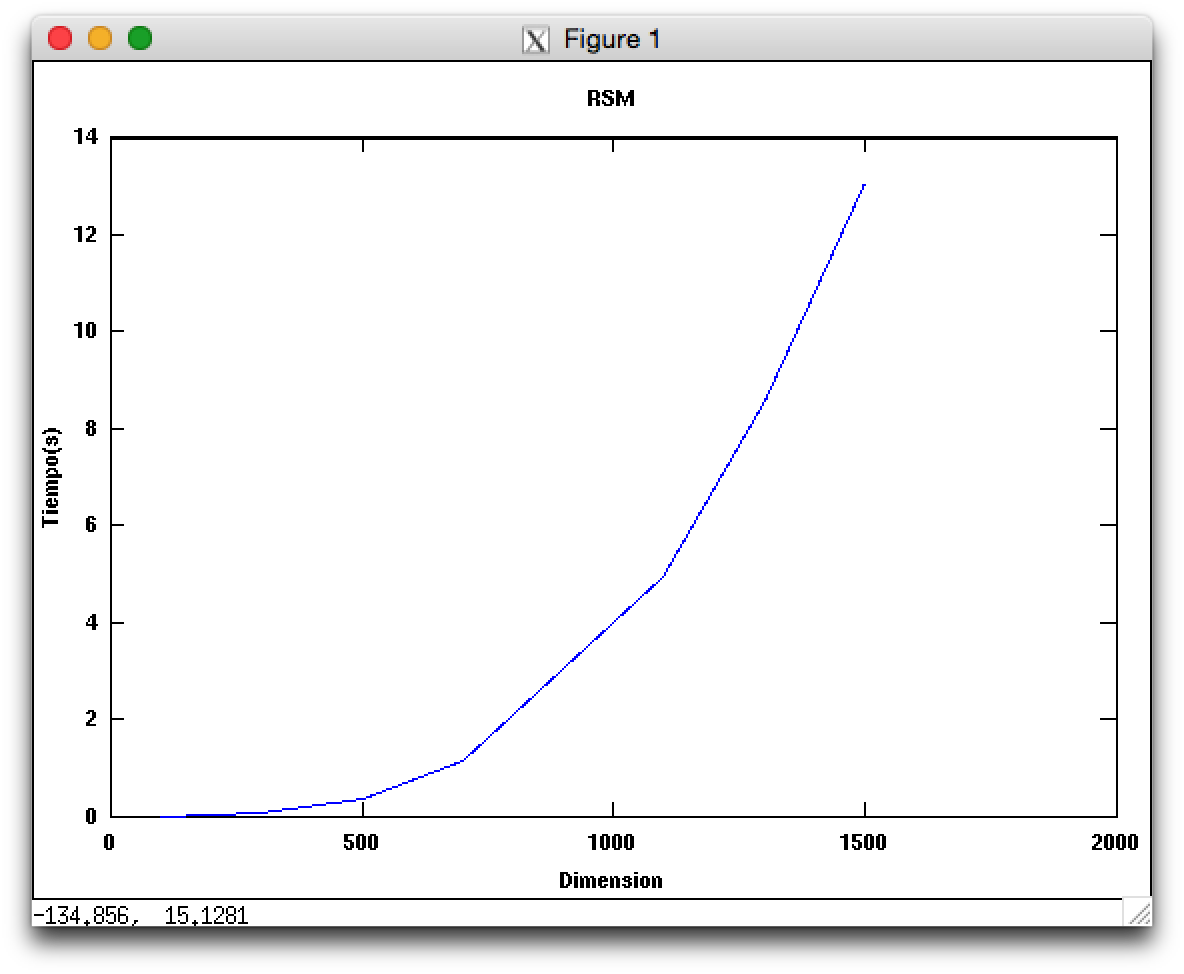
\includegraphics[width=100mm]{GenerateRSM.png} 

Si bien durante las primeras implementaciones pudimos obtener correctamente los autovalores de cualquier tipo de matriz, los tiempos son considerablemente mayores a los de la función \texttt{eig} de Octave.

Los resultados obtenidos se muestran en el Cuadro 1:

\begin{center}
\begin{table}[h]
\centering
\begin{tabular}{cc}
\hline
\textbf{Dimensión (nxn)} & \textbf{Tiempo (ms)} \\ \hline
5                  & 33                 \\
15                 & 74                 \\
30                 & 4475                 \\
50                 & 21393                \\
100                & 243651
\end{tabular}
\caption[Texto del índice (opcional)]{Tiempo transcurrido del cálculo de autovalores en base a la dimensión N de la matriz.}
\end{table}
\end{center}

Si bien obtuvimos una implementación donde el método QR implementado funciona para cualquier matriz cuadrada vamos en la próxima iteración a aprovechar la gran cantidad de ceros de la matriz GRCAR para bajar considerablemente los tiempos y obtener una implementación que calcule los autovalores sólo a una matriz rala.

Los resultados obtenidos con esta nueva implementación se muestran en el Cuadro 2:

\begin{center}
\begin{table}[!htbp]
\centering
\begin{tabular}{cc}
\hline
\textbf{Dimensión (nxn)} & \textbf{Tiempo (ms)} \\ \hline
5                  & 38                \\
15                 & 251                \\
30                 & 4461                 \\
50                 & 20964                \\
100                & 233487
\end{tabular}
\caption[Texto del índice (opcional)]{Tiempo transcurrido del cálculo de autovalores en base a la dimensión N de la matriz con las mejoras de procesamiento de matriz rala.}
\end{table}
\end{center}


Como se puede ver, el tiempo transcurrido en matrices de tamaño considerable es menor que en la implementación previa. Sin embargo, los mismos siguen siendo considerablemente mayores que los del octave. Para una dimensión de 200 el programa terminaba por la cantidad de iteraciones y el error con respecto al valor real era mayor al elegido. Con matrices mas grandes, de 500x500 por ejemplo, nuestro programa ni siquiera llega a devolver un valor. En cambio, si uno prueba la matriz en octave el resultado es devuelto en cuestión de segundos.


\section{Conclusiones}
Como conclusión, logramos obtener correctamente los autovalores de una matriz GRCAR de hasta una dimensión de un n=100. Viendo los tiempos transcurridos en nuestra implementación, podemos deducir que un lenguaje de alto nivel como java no fue la mejor elección a la hora de trabajar con matrices de gran dimensión. Hay que tener en cuenta que utilizamos nuestras propias implementaciones de funciones necesarias para el manejo de matrices y vectores, las cuales en eficiencia no están a la altura de las de un lenguaje de programación con funciones matemáticas pre-programadas (octave).

\pagebreak

\section{Bibliografía}
\begin{itemize}

\item Apuntes de las clases teórica y práctica de la materia Métodos Numéricos Avanzados (Segundo Cuatrimestre, 2015).

\item Documento sobre descomposición QR proporcionado por la cátedra de Métodos Numéricos Avanzados (Segundo Cuatrimestre, 2015).

\item \url{http://www.win.tue.nl/casa/meetings/seminar/previous/_abstract051109_files/presentation_full.pdf}

\item \url{http://people.inf.ethz.ch/arbenz/ewp/Lnotes/chapter3.pdf}

\end{itemize}

\pagebreak

\begin{large}
ANEXO
\end{large}

\begin{center}
\textbf{Vector.java}
\end{center}

\begin{verbatim}

package grcar;

/**
 * Clase auxiliar para el manejor de matrices double[][] y vectores double[]. *
 */
public class Vector {

	/**
	 * Suma Vectorial
	 * @param v1 : Vector double[]
	 * @param v2 : Vector double[]
	 * @return Vector suma v1() + v2()
	 */
	public static double[] sumVec(double[] v1, double[] v2) {
		double[] res = new double[v1.length];
		for (int i = 0; i < v1.length; i++) {
			res[i] = v1[i] + v2[i];
		}
		return res;
	}

	/**
	 * Método para obtener la n-ésima columna de una matriz.
	 * @param m : Matriz double[]
	 * @param n : índice n de la columna (0 =< n <= col(m))
	 * @return La n-ésima columna de la matriz m
	 */
	public static double[] getColumn(double[][] m, int n) {
		double[] res = new double[m.length];
		for (int i = 0; i < m.length; i++) {
			res[i] = m[i][n];
		}
		return res;
	}

	/**
	 * Producto entre vector V y escalar X
	 * @param v : Vector double[]
	 * @param x : Escalar double
	 * @return Vector x * v()
	 */
	public static double[] prodVectEsc(double[] v, double x) {
		double[] res = new double[v.length];
		for (int i = 0; i < v.length; i++) {
			res[i] = v[i] * x;
		}
		return res;
	}

	/**
	 * Producto Interno entre vectores
	 * @param x : Vector double[]
	 * @param y : Vector double[]
	 * @return Producto Interno <x,y>
	 */
	public static double prodInt(double[] x, double[] y) {
		double[][] auxx = new double[1][x.length];
		double[][] auxy = new double[1][y.length];
		auxx[0] = x;
		auxy[0] = y;
		return matrixprod(auxy, traspose(auxx))[0][0];
	}

	/**
	 * Norma 2 de un vector
	 * @param v : Vector double[]
	 * @return Norma 2 del vector v
	 */
	public static double norm2(double[] v) {
		double aux = 0;
		for (double x : v) {
			aux += x * x;
		}
		return Math.sqrt(aux);
	}

	/**
	 * Producto entre matrices
	 * @param m1 : Matriz double[][]
	 * @param m2 : Matriz double[][]
	 * @return Matriz m1 * m2
	 */
	public static double[][] matrixprod(double[][] m1, double[][] m2) {
		double[][] res = new double[m1.length][m2[0].length];
		if (m1[0].length != m2.length) {
			return null;
		}
		for (int i = 0; i < res.length; i++) {
			for (int j = 0; j < res[0].length; j++) {
				double aux = 0;
				for (int k = 0; k < m1[0].length; k++) {
					aux += (m1[i][k] * m2[k][j]);
				}
				res[i][j] = aux;
			}
		}
		return res;
	}

	/**
	 * Método del determinante.
	 * @param mat : Una matriz cuadrada double[][]
	 * @return El determinante de la matriz mat
	 */
	public static double determinant(double[][] mat) {
		double result = 0;
		if (mat.length == 2) {
			result = mat[0][0] * mat[1][1] - mat[0][1] * mat[1][0];
			return result;
		}
		for (int i = 0; i < mat[0].length; i++) {
			double temp[][] = new double[mat.length - 1][mat[0].length - 1];
			for (int j = 1; j < mat.length; j++) {
				System.arraycopy(mat[j], 0, temp[j - 1], 0, i);
				System.arraycopy(mat[j], i + 1, temp[j - 1], i, mat[0].length
						- i - 1);
			}
			if (mat[0][i] != 0) {
				result += mat[0][i] * Math.pow(-1, i) * determinant(temp);
			}
		}
		return result;
	}

	/**
	 * Traspuesta de una matriz
	 * @param mat : Una matriz double[][]
	 * @returnLa traspuesta de la matriz mat
	 */
	public static double[][] traspose(double[][] mat) {
		double[][] aux = new double[mat[0].length][mat.length];
		for (int i = 0; i < mat[0].length; i++)
			for (int j = 0; j < mat.length; j++)
				aux[i][j] = mat[j][i];
		return aux;
	}

	/**
	 * Método para imprimir una matriz double[][]
	 * @param matrix : Matriz a imprimir en pantalla
	 */
	public static void printMatrix(double[][] matrix) {
		for (int i = 0; i < matrix.length; i++) {
			for (int j = 0; j < matrix[0].length; j++) {
				if (matrix[i][j] < 0) {
					System.out.printf(" %.5f", matrix[i][j]);
				} else {
					System.out.printf("  %.5f", matrix[i][j]);
				}
			}
			System.out.println();
		}
	}
}

\end{verbatim}

\begin{center}
\textbf{Complex.java}
\end{center}

\begin{verbatim}
package grcar;

import java.util.ArrayList;
import java.util.List;

/**
 * Clase auxiliar creada para el manejo de valores complejos.
 */
public class Complex {

	private double real;
	private double img;

	public Complex(double real, double img) {
		this.real = real;
		this.img = img;
	}

	@Override
	public String toString() {
		String realstring = String.format("%.5f", real);
		String imgstring = String.format("%.5f", Math.abs(img));
		if (img >= 0)
			return realstring + " + " + imgstring + "i";
		return realstring + " - " + imgstring + "i";
	}

	public Complex conjugate() {
		return new Complex(real, -img);
	}

	public double mod() {
		return Math.sqrt(real * real + img * img);
	}

	public double getReal(){
		return real;
	}

	/**
	 * Fórmula Resolvente Cuadrática
	 * @param a Coeficiente de grado 2
	 * @param b	Coeficiente de grado 1
	 * @param c Coeficiente de grado 0
	 * @return Las raíces del polinomnio de grado 2 ax^2 + bx + c (Reales y Complejas).
	 */
	public static List<Complex> roots(double a, double b, double c) {
		List<Complex> res = new ArrayList<Complex>();
		double x = (b * b) - (4 * a * c);
		if (x > 0) {
			res.add(0, new Complex(((-b + Math.sqrt(x)) / 2 * a), 0));
			res.add(1, new Complex(((-b - Math.sqrt(x)) / 2 * a), 0));
		} else {
			res.add(0, new Complex(-b / (2 * a), Math.sqrt(Math.abs(x))
					/ (2 * a)));
			res.add(1, res.get(0).conjugate());
		}
		return res;
	}
}

\end{verbatim}

\begin{center}
\textbf{Grcar.java}
\end{center}

\begin{verbatim}
package grcar;

import java.util.ArrayList;
import java.util.HashMap;
import java.util.List;
import java.util.Map;

public class Grcar {

	private static final double E = 0.0001;
	private static final long MAX_ITERATIONS = 10000;
	private static final int CHECK_FREQUENCY = 1;

	/**
	 * Consigna A. Obtener la matriz Grcar de NxN
	 * @param n : Dimensión de la Matriz Grcar a obtener
	 * @return Matriz Grcar double[n][n]
	 */
	public static double[][] getGrcarMatrix(int n) {
		int k = 3;
		double[][] matrix = new double[n][n];
		for (int i = 0; i < n; i++) {
			for (int j = 0; j < n; j++) {
				if (i == j) {
					matrix[i][j] = 1;
				} else if (i == (j + 1)) {
					matrix[i][j] = -1;
				} else if (j > i && j <= (i + k)) {
					matrix[i][j] = 1;
				} else {
					matrix[i][j] = 0;
				}
			}
		}
		return matrix;
	}

	/**
	 * Optimización del método matrixprod para el caso especial
	 * con m1 = R y m2 = q de la descomposición QR.
	 * @param r : Matriz R de la descomposición QR.
	 * @param q : Matriz Q de la descomposición QR.
	 * @return Matriz R * Q
	 */
	public static double[][] matrixRprodQ(double[][] r, double[][] q) {
		double[][] res = new double[r.length][q[0].length];
		for (int i = 0; i < res.length; i++) {
			for (int j = 0; j < res[0].length; j++) {
				double aux = 0;
				for (int k = i; k < r[0].length && k <= 2*(Math.floor(j/2)+1); k++) {
					aux += (r[i][k] * q[k][j]);
				}
				res[i][j] = aux;
			}
		}
		return res;
	}

	/**
	 * Descomposición QR de la matriz m.
	 * @param m : Matriz double[][]
	 * @return Mapa que contiene las matrices Q y R de la descomposición QR de la matriz m.
	 * <"Q", Matriz Q>
	 * <"R", Matrix R>
	 */
	public static Map<String, double[][]> QR(double[][] m) {
		Map<String, double[][]> res = new HashMap<String, double[][]>();
		double[][] Q = new double[m.length][m.length];
		double[][] R = new double[m.length][m[0].length];
		List<double[]> q = new ArrayList<double[]>();
		for (int k = 0; k < m[0].length; k++) {
			double[] v = Vector.getColumn(m, k);
			double[] e = v;
			for (int n = 0; n < q.size(); n++) {
				double p = Vector.prodInt(v, q.get(n));
				e = Vector.sumVec(e, Vector.prodVectEsc(q.get(n), -p));
				R[n][k] = p;
			}
			double norm2e = Vector.norm2(e);
			R[k][k] = norm2e;
			e = Vector.prodVectEsc(e, 1 / norm2e);
			q.add(e);
			for (int i = 0; i < e.length; i++)
				Q[i][k] = e[i];
		}
		res.put("Q", Q);
		res.put("R", R);
		return res;
	}

	/**
	 * Método para el cálculo de autovalores de la matriz m
	 * @param m : Matriz double[][]
	 * @return Lista con los autovalores (reales y complejos) de la matriz m
	 */
	public static List<Complex> eig(double[][] m) {
		List<Complex> eigs = new ArrayList<Complex>();
		if (m.length == 2 && m[0].length == 2)
			return Complex.roots(1, -m[0][0] - m[1][1], Vector.determinant(m));
		double [] dets = new double[(m.length)/2];
		double[][] T = m;
		boolean flag = false;
		for (int k = 0; k < MAX_ITERATIONS && !flag; k++) {
			Map<String, double[][]> qr = QR(T);
//			T = matrixprod(matrixprod(traspose(qr.get("Q")),T),qr.get("Q"));
			T = matrixRprodQ(qr.get("R"), qr.get("Q"));
//			T = matrixprod(qr.get("R"), qr.get("Q"));
			if( k % (m.length*CHECK_FREQUENCY) == 0){
				double[][] current = new double[2][2];
				flag = true;
				for (int i = 0; i < m.length - m.length % 2; i += 2) {
					current[0][0] = T[i][i];
					current[0][1] = T[i][i + 1];
					current[1][0] = T[i + 1][i];
					current[1][1] = T[i + 1][i + 1];
					double currentdet = Vector.determinant(current);
					if(Math.abs(dets[i/2]-currentdet) > E){
						flag = false;
					}
					dets[i/2]=currentdet;
				}
			}
		}
		for (int i = 0; i < m.length - m.length % 2; i += 2) {
			double[][] aux = new double[2][2];
			aux[0][0] = T[i][i];
			aux[0][1] = T[i][i + 1];
			aux[1][0] = T[i + 1][i];
			aux[1][1] = T[i + 1][i + 1];
			eigs.addAll(eig(aux));
		}
		if (m.length % 2 == 1) {
			eigs.add(new Complex(T[T.length - 1][T.length - 1], 0));
		}
		return eigs;
	}

	public static void main(String[] args) {
		long init = System.currentTimeMillis();
		int n = 10;
		System.out.println("GRCAR " + n + "x" + n);
		double[][] grcar = getGrcarMatrix(n);
		System.out.println("\nAutovalores");
		List<Complex> eigs = eig(grcar);
		for (Complex e : eigs) {
			System.out.println(e);
		}
		long end = System.currentTimeMillis();
		System.out.println("\nTiempo transcurrido: " + (end - init) + " milisegundos");
	}
}

\end{verbatim}

\end{document}